\documentclass{standalone}
\usepackage{tikz}
\usetikzlibrary{patterns}
\usepackage{siunitx}
\begin{document}
	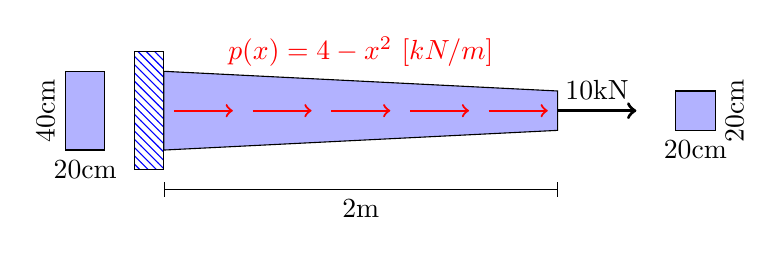
\begin{tikzpicture}[scale=2.5]
		\draw[pattern=north west lines, pattern color=blue] (-.15, -.3) rectangle (0, .3);
		\draw[fill=blue!30] (0,-.2) -- (0, .2) -- (2, .1) -- (2, -.1) -- cycle;
		\draw[|-|] (0, -.4) -- (2, -.4) node[pos=.5, below] {$2\unit{m}$};
		
		% Sección izq
		\draw[fill=blue!30] (-.5, -.2) rectangle (-.3, .2);
		\node at (-.4, -.3) {$20 \unit{cm}$};
		\node[rotate=90] at (-.6, 0) {$40 \unit{cm}$};
		
		% Sección der
		\draw[fill=blue!30] (2.6, -.1) rectangle (2.8, .1);
		\node at (2.7, -.2) {$20 \unit{cm}$};
		\node[rotate=90] at (2.9, 0) {$20 \unit{cm}$};
		
		% Carga distribuida
		\foreach \x in {0.05, .45, .85, 1.25, 1.65}{
			\draw[->, red, thick] (\x, 0) -- (\x + .3, 0);}
		\node[red] at (1, .3) {$p(x) = 4 - x^2 \ [kN/m]$};
		\draw[->, very thick] (2, 0) -- (2.4, 0) node[pos=.5, above]{$10\unit{kN}$};
	\end{tikzpicture}
\end{document}